%%% The main file. It contains definitions of basic parameters and includes all other parts.

%% Settings for single-side (simplex) printing
% Margins: left 40mm, right 25mm, top and bottom 25mm
% (but beware, LaTeX adds 1in implicitly)
\documentclass[12pt,a4paper]{report}
\setlength\textwidth{145mm}
\setlength\textheight{247mm}
\setlength\oddsidemargin{15mm}
\setlength\evensidemargin{15mm}
\setlength\topmargin{0mm}
\setlength\headsep{0mm}
\setlength\headheight{0mm}
% \openright makes the following text appear on a right-hand page
\let\openright=\clearpage

%% Settings for two-sided (duplex) printing
% \documentclass[12pt,a4paper,twoside,openright]{report}
% \setlength\textwidth{145mm}
% \setlength\textheight{247mm}
% \setlength\oddsidemargin{14.2mm}
% \setlength\evensidemargin{0mm}
% \setlength\topmargin{0mm}
% \setlength\headsep{0mm}
% \setlength\headheight{0mm}
% \let\openright=\cleardoublepage

%% Generate PDF/A-2u
\usepackage[a-2u]{pdfx}

%% Character encoding: usually latin2, cp1250 or utf8:
\usepackage[utf8]{inputenc}

%% Prefer Latin Modern fonts
\usepackage{lmodern}

%% Further useful packages (included in most LaTeX distributions)
\usepackage{amsmath}        % extensions for typesetting of math
\usepackage{amsfonts}       % math fonts
\usepackage{amsthm}         % theorems, definitions, etc.
\usepackage{bbding}         % various symbols (squares, asterisks, scissors, ...)
\usepackage{bm}             % boldface symbols (\bm)
\usepackage{graphicx}       % embedding of pictures
\usepackage{fancyvrb}       % improved verbatim environment
\usepackage{natbib}         % citation style AUTHOR (YEAR), or AUTHOR [NUMBER]
\usepackage[nottoc]{tocbibind} % makes sure that bibliography and the lists
			    % of figures/tables are included in the table
			    % of contents
\usepackage{dcolumn}        % improved alignment of table columns
\usepackage{booktabs}       % improved horizontal lines in tables
\usepackage{paralist}       % improved enumerate and itemize
\usepackage{xcolor}         % typesetting in color

% Path to images folder
\graphicspath{ {./images/} }

%%% Basic information on the thesis

% Thesis title in English (exactly as in the formal assignment)
\def\ThesisTitle{Thesis title}

% Author of the thesis
\def\ThesisAuthor{Name Surname}

% Year when the thesis is submitted
\def\YearSubmitted{YEAR}

% Name of the department or institute, where the work was officially assigned
% (according to the Organizational Structure of MFF UK in English,
% or a full name of a department outside MFF)
\def\Department{Name of the department}

% Is it a department (katedra), or an institute (ústav)?
\def\DeptType{Department}

% Thesis supervisor: name, surname and titles
\def\Supervisor{Supervisor's Name}

% Supervisor's department (again according to Organizational structure of MFF)
\def\SupervisorsDepartment{department}

% Study programme and specialization
\def\StudyProgramme{study programme}
\def\StudyBranch{study branch}

% An optional dedication: you can thank whomever you wish (your supervisor,
% consultant, a person who lent the software, etc.)
\def\Dedication{%
Dedication.
}

% Abstract (recommended length around 80-200 words; this is not a copy of your thesis assignment!)
\def\Abstract{%
Abstract.
}

% 3 to 5 keywords (recommended), each enclosed in curly braces
\def\Keywords{%
{key} {words}
}

%% The hyperref package for clickable links in PDF and also for storing
%% metadata to PDF (including the table of contents).
%% Most settings are pre-set by the pdfx package.
\hypersetup{unicode}
\hypersetup{breaklinks=true}

% Definitions of macros (see description inside)
%%% This file contains definitions of various useful macros and environments %%%
%%% Please add more macros here instead of cluttering other files with them. %%%

%%% Minor tweaks of style

% These macros employ a little dirty trick to convince LaTeX to typeset
% chapter headings sanely, without lots of empty space above them.
% Feel free to ignore.
\makeatletter
\def\@makechapterhead#1{
  {\parindent \z@ \raggedright \normalfont
   \Huge\bfseries \thechapter. #1
   \par\nobreak
   \vskip 20\p@
}}
\def\@makeschapterhead#1{
  {\parindent \z@ \raggedright \normalfont
   \Huge\bfseries #1
   \par\nobreak
   \vskip 20\p@
}}
\makeatother

% This macro defines a chapter, which is not numbered, but is included
% in the table of contents.
\def\chapwithtoc#1{
\chapter*{#1}
\addcontentsline{toc}{chapter}{#1}
}

% Draw black "slugs" whenever a line overflows, so that we can spot it easily.
\overfullrule=1mm

%%% Macros for definitions, theorems, claims, examples, ... (requires amsthm package)

\theoremstyle{plain}
\newtheorem{thm}{Theorem}
\newtheorem{lemma}[thm]{Lemma}
\newtheorem{claim}[thm]{Claim}

\theoremstyle{plain}
\newtheorem{defn}{Definition}

\theoremstyle{remark}
\newtheorem*{cor}{Corollary}
\newtheorem*{rem}{Remark}
\newtheorem*{example}{Example}

%%% An environment for proofs

\newenvironment{myproof}{
  \par\medskip\noindent
  \textit{Proof}.
}{
\newline
\rightline{$\qedsymbol$}
}

%%% An environment for typesetting of program code and input/output
%%% of programs. (Requires the fancyvrb package -- fancy verbatim.)

\DefineVerbatimEnvironment{code}{Verbatim}{fontsize=\small, frame=single}

%%% The field of all real and natural numbers
\newcommand{\R}{\mathbb{R}}
\newcommand{\N}{\mathbb{N}}

%%% Useful operators for statistics and probability
\DeclareMathOperator{\pr}{\textsf{P}}
\DeclareMathOperator{\E}{\textsf{E}\,}
\DeclareMathOperator{\var}{\textrm{var}}
\DeclareMathOperator{\sd}{\textrm{sd}}

%%% Transposition of a vector/matrix
\newcommand{\T}[1]{#1^\top}

%%% Various math goodies
\newcommand{\goto}{\rightarrow}
\newcommand{\gotop}{\stackrel{P}{\longrightarrow}}
\newcommand{\maon}[1]{o(n^{#1})}
\newcommand{\abs}[1]{\left|{#1}\right|}
\newcommand{\dint}{\int_0^\tau\!\!\int_0^\tau}
\newcommand{\isqr}[1]{\frac{1}{\sqrt{#1}}}

%%% Various table goodies
\newcommand{\pulrad}[1]{\raisebox{1.5ex}[0pt]{#1}}
\newcommand{\mc}[1]{\multicolumn{1}{c}{#1}}


% Title page and various mandatory informational pages
\begin{document}
%%% Title page of the thesis and other mandatory pages

%%% Title page of the thesis

\pagestyle{empty}
\hypersetup{pageanchor=false}
\begin{center}

\centerline{\mbox{
\includegraphics[width=166mm]{./logo-en.pdf}}}

\vspace{-8mm}
\vfill

{\bf\Large BACHELOR THESIS}

\vfill

{\LARGE\ThesisAuthor}

\vspace{15mm}

{\LARGE\bfseries\ThesisTitle}

\vfill

\Department

\vfill

{
\centerline{\vbox{\halign{\hbox to 0.45\hsize{\hfil #}&\hskip 0.5em\parbox[t]{0.45\hsize}{\raggedright #}\cr
Supervisor of the bachelor thesis:&\Supervisor \cr
\noalign{\vspace{2mm}}
Study programme:&\StudyProgramme \cr
\noalign{\vspace{2mm}}
Study branch:&\StudyBranch \cr
}}}}

\vfill

% Zde doplňte rok
Prague \YearSubmitted

\end{center}

\newpage

%%% Here should be a bound sheet included -- a signed copy of the "bachelor
%%% thesis assignment". This assignment is NOT a part of the electronic
%%% version of the thesis. DO NOT SCAN.

%%% A page with a solemn declaration to the bachelor thesis

\openright
\hypersetup{pageanchor=true}
\pagestyle{plain}
\pagenumbering{roman}
\vglue 0pt plus 1fill

\noindent
I declare that I carried out this bachelor thesis independently, and only with the cited
sources, literature and other professional sources. It has not been used to obtain another
or the same degree.

\medskip\noindent
I understand that my work relates to the rights and obligations under the Act No.~121/2000 Sb.,
the Copyright Act, as amended, in particular the fact that the Charles
University has the right to conclude a license agreement on the use of this
work as a school work pursuant to Section 60 subsection 1 of the Copyright~Act.

\vspace{10mm}

\hbox{\hbox to 0.5\hsize{%
In \hbox to 6em{\dotfill} date \hbox to 6em{\dotfill}
\hss}\hbox to 0.5\hsize{\dotfill\quad}}
\smallskip
\hbox{\hbox to 0.5\hsize{}\hbox to 0.5\hsize{\hfil Author's signature\hfil}}

\vspace{20mm}
\newpage

%%% Dedication

\openright

\noindent
\Dedication

\newpage

%%% Mandatory information page of the thesis

\openright

\vbox to 0.5\vsize{
\setlength\parindent{0mm}
\setlength\parskip{5mm}

Title:
\ThesisTitle

Author:
\ThesisAuthor

\DeptType:
\Department

Supervisor:
\Supervisor, \SupervisorsDepartment

Abstract:
\Abstract

Keywords:
\Keywords

\vss}

\newpage

\openright
\pagestyle{plain}
\pagenumbering{arabic}
\setcounter{page}{1}


%%% A page with automatically generated table of contents of the bachelor thesis

\tableofcontents

%%% Each chapter is kept in a separate file
\chapter*{Introduction}
\addcontentsline{toc}{chapter}{Introduction}

% his speech does not  flow in a natural way - nie je pravda , je to naopak
Imagine, for a moment, that you are transported in time to 10th-century Europe. It is Sunday, and the weekly mass is just
starting. Look around yourself. The tall ceilings of the impressive church were built so to bring you closer to God. The stained glass windows
let through just enough light so that it is not completely dark. Can you smell the incense? Everything in the environment around
you reminds you that you are taking part in a sacred ritual. Listen to the priest; when he recites the prayers, his speech does not 
flow in a natural way. Instead, the entire text is intoned on a single note, except for the slightly inflected ends of clauses. 
Sometimes, the choir replaces the priest, singing more elaborate monophonic melodies. The words they are singing are Latin, but even 
if you do not understand them, you know what their purpose is: to celebrate the deity. Their voices echo in the stone church, creating an
otherwordly experience.

What you are hearing is called emph{Gregorian chant}, one of the oldest preserved types of music. It has been central to the cultural development
of most of Europe, as it is a part of the Roman-catholic tradition. Figure \ref{fig:chant_manuscripts} shows an example of four chants
\footnote{\url{http://www.ksbm.oeaw.ac.at/images/AT/5000/AT5000-1011/AT5000-1011\_1v.jpg}}\footnote{\url{http://www.uni-regensburg.de/Fakultaeten/phil\_Fak\_I/Musikwissenschaft/cantus/microfilm/copenhagen/vol3/images/008.jpg}}\footnote{\url{http://manuscripta.at/diglit/AT5000-589/09}}\footnote{\url{https://gallica.bnf.fr/ark:/12148/btv1b10033588d/f5.image}} as they are found in
the original manuscripts. The chant in the upper right corner uses notation which is not dissimilar from contemporary musical notation,
while the chant in the lower right image only uses memory aids without the exact pitch. This highlights the differences
between the ways chant was recorded over the centuries (see Section \ref{section:notation}).

\begin{figure}[h]
\centering
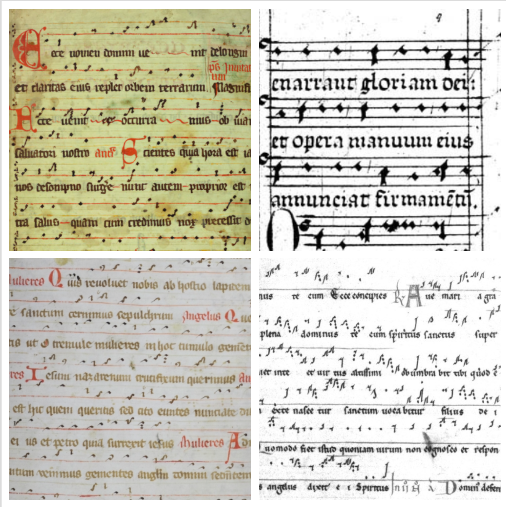
\includegraphics{chant_manuscripts}
\caption{An example of chants as inscribed in manuscripts.}
\label{fig:chant_manuscripts}
\end{figure}

Gregorian chant is a widely researched topic of study, partly thanks to the substantial amount of available sources. However, traditional
musicology is limited by the individual capacity; it is infeasible to study extremely large numbers of chants by hand. This is where
Digital Humanities come into play. Digitalization of large corpora of Gregorian chant enables researchers to draw conclusions
supported by much more data than a human could ever examine.

Nevertheless, contemporary Gregorian chant research still lacks software tools that would facilitate the study of chant repertoire. An example
of an important problem is chant's historical and geographical development. Throughout the 
centuries, the tradition spread accross Europe, while always changing a small part of it. This has led to many variations of the same
chants existing at the same time. Knowing how exactly the changes came into place could shed light on many open questions in the history of 
European culture.

\textbf{The aim of this thesis is to create a tool that musicologists could use to answer questions about chant origin and evolution.} We do this by employing
well-known algorithms for multiple sequence alignment from bioinformatics. Once the idea is proposed, it is almost immediately obvious that
biological and musical sequences share features which warrant using the same methods on both. As opposed to other sequence comparison techniques, such as edit
distance, MSA algorithms do not need any assumptions about the length of chants or other characteristics, which is why they are suitable
for the study of chant.

% screenshot alignmentu s conservation profilom

The tool provides the ability to align a set of chants that is potentially large and diverse in multiple ways, each of which has slightly different uses. One important
implication of the tool is that it makes the discovery contrafacta (chants with the same melody but different lyrics) and transpositions
(chants with the same melody but shifted by an interval) across large repertoires easy.

It is important to note that the purpose of this thesis is not to conduct experiments. It is merely a tool for musicologists who possess
the knowledge needed to select the appropriate data so that previously infeasible discoveries can be made.


\chapter{Related work}

With the advent of computers, the field of Music Information Retrieval (MIR) emerged. Research in this interdisciplinary field focuses on extracting
information from musical notation using computer science methods, such as signal processing or machine learning. Its applications
vary widely, from recommender systems, to automatic audio transcription, to music generation. MIR encompasses all different kinds of music,
regardless of their location, age, or function. Researchers have developed a multitude of software tools that facilitate music analysis,
irrespective of what type of music it is. One of such toolkits is \emph{music21} \citep{music21}, a Python package able to encode musical notation
as Python objects and perform analysis on large datasets.

The study of plainchant using computational methods has not been done extensively. The main research tool for musicologists in this field
is the Cantus Index \citep{cantus_index}. It is an online index of chants from several different chant databases, providing researchers with 
a common API for all of them. The entries in Cantus Index only contain four data fields: full-text, genre, feast (not required), and Cantus ID,
which is automatically assigned to newly added chants. The tool is also able to search for melodies in the original source and even provides 
search-by-melody functionality. There are ten databases indexed in the catalogue, the largest of which is the Cantus database \citep{cantus_db}.

\cite{chant21} developed \emph{chant21}, a Python package able to convert two standard melodic notations, \emph{volpiano} and \emph{gabc} to
a \emph{music21} object, therefore making it easier to study Gregorian chant computationally. The data they used were 
scraped from Cantus database \citep{cantus_db} and GregoBase \citep{gregobase} and released as CantusCorpus and GregoBaseCorpus, respectively.
Finally, they performed two case studies using the package. In the first one, they confirmed the melodic arch hypothesis \citep{melodic_arch}, 
which had previously only been studied manually. Second, they analyzed the relation between differentiæ and antiphon openings \citep{differentiae}
and found that it differs accross modes.

Some of the computational research into plainchant has been centered on mode classification. \cite{mode_huron} used pitch class profiles to
classify modes. They created a pitch-class distribution for each of the eight modes, and used these classes to classify previously unseen data.
\cite{mode_cornelissen} compared three approaches to mode classification: classical approach, which classifies chants based on
the final pitch, range, and the initial pitch; profile approach, which was largely inspired by \cite{mode_huron}; and distributional approach,
which focuses on the melodic aspect of mode. The authors chose various segmentations and representations of chants and used a tf-idf vector
model to classify mode. The study found that we can accurately classify mode even when we discard all absolute pitch information, the melody
contour contains enough information on its own.

A considerable amount of research has been done into the evaluation of melodic similarity, albeit not for Gregorian chant specifically.
\cite{melodic_similarity} provides an overview of the methods. He mentions edit distance, Markov chains, and geometric measurements as
the most widely used ones. \cite{similarity_plot} used an adapted edit distance metric to calculate the similarity of two melodic sequences
by first calculating the similarity for all segments of each of the sequences and then scaling them by a weight function depending on the
segment length, which yielded them what they call a multi-scale similarity stack. The overall similarity was obtained by averaging its values.
Then they used the MSS stack to create a visualization that takes on the shape of a trapezoid that shows which segments of two sequences
are the most similar.

\cite{similarity_bioinf} argue that methods originally developed for bioinformatics have a great potential to be applied to music. They offer
analogies for bioinformatics concepts found in musicology. For example, they liken DNA and proteins to melodic sequences, homologues (proteins that
have the same ancestor) to song covers, evolution to oral transmission, etc. They claim that despite the similarities, MRI has not leveraged the
full potential of bioinformatics methods. In their article, they focus on modelling melodic similarity using multiple-sequence alignment (MSA)
algorithms, therefore not relying on heuristics, as opposed to previous works. Their results revealed that the MAFFT algorithm yields the best
alignemnt, which can be attributed to the algorithm using gap-free segments as anchor points, therefore partitioning melodies into more meaningful
segments than other algorithms.

The general algorithm for calculating pairwise sequence alignment is the Needleman-Wunsch algorithm \citep{needleman}. It uses dynamic programming
to break down the problem into smaller problems. Given two sequences, it starts aligning them from the beginning. At each point, the algorithm checks
whether the two sequences match in the current position, and if not, whether it will leave the elements mismatched or insert a space. In essence,
all possible alignments are computed and scored and the best one is chosen. The algorithm always yields an optimal alignment, therefore it is
used when the quality of the alignment is important. However, because of its time complexity, it is unsuitable for many applications.

Unlike pairwise sequence alignment, multiple sequence alignment has been shown to be NP-complete \citep{msa_complexity}. As such, there is no practical
way of computing an optimal MSA and we must instead rely on heuristics to obtain a sufficiently good alignment.

\cite{msa_overview} provides an overview of modern multiple sequence alignment algorithms. According to him, the most frequently used algorithms use
the progressive approach, where a guide tree is estimated from unaligned sequences and then pairwise alignment algorithms are used to find
the MSA following the tree. He notes that the scoring methods of the pairwise algorithm are essential. There are two main groups of scoring methods:
matrix-based algorithms, where a substitution matrix is used to determine the cost of replacing one symbol with another, and the consistency-based
methods, which use a collection of global and local alignments to calculate a position-specific substitution matrix. The author claims that
the best methods yield indistinguishable results, except for remote homologs with less than 25\% identity.

T-Coffee \citep{t_coffee} uses the progressive approach described above. It was the first algorithm that used a preprocessed collection of 
alignments to create a library that helps create the guide tree. The library is generated using both global and local pairwise alignments.
Thanks to this approach, T-Coffee minimizes the errors made in the first stages of building the MSA, which is a shortcoming of many previous
algorithms, as these errors tend to persist. They combined precomputed local and global alignments and create a function that assigns a weight to
each pairwise alignment depending on how consistent the pair of residues is with the residue pairs from all other alignments. This process
leads to a significant improvement of the results.

MAFFT \citep{mafft} further improves on other methods by using Fast Fourier transform to identify homologues fast. In addition, the authors
propose a simplified scoring system that reduces CPU time while maintaining its accuracy. The authors' results showed a performance 
100 times better than that of T-Coffee. 

Despite the fact that MSA algorithms have already been used for music analysis, this is the first work that focuses specifically on applying
the methods on Gregorian chant. Gregorian chant is specific by its monophonic nature, which means that there is just one sequence to analyze.
Each chant has also undergone many changes over the centuries, therefore there are many variants of the same chants that can be
researched. These characteristics make Gregorian chant an ideal subject for MSA analysis and subsequent application of related bioinformatics methods.

% one sequence to analyze (as is the case of modern repertoire)

\chapter{Data}

Our main source of data is the Cantus database (\cite{cantus_db}), one of the databases indexed in the Cantus Index. The database serves as a 
digital archive of chants, each entry containing information about its source, liturgical occasion, mode, and others. Work on the project started
in the late 1980s, and to date, around 500,000 individual chants from approximately 150 manuscripts have been indexed. Each entry is transcribed 
manually and undergoes a thorough examination before publishing (\cite{cantus_lacoste}).

We are using a scraped version of the Cantus database released as CantusCorpus (\cite(chant21)). Unlike the Cantus database which is continuously being
updated and is therefore unsuitable for computational study, the corpus is versioned, therefore each version always contains the same data. We are using
version 0.2 released in July 2020 which contains 497071 entries. The corpus is available for download in CSV format.

\section{CSV}

CSV is one of the most common formats for tabular data. The abbreviation stands for \emph{comma-separated values}. As the name suggests, the format
uses commas to separate columns (although other separators, such as a semicolon, can be used as well to allow for simpler parsing in case that the data 
frequently contains commas that would otherwise need to be escaped), while the individual rows are separated by a line break. The data is stored as plaintext,
which makes it easily readable. Parsing CSV files becomes more complicated when the data contains column and row separators inside fields; in that case
quotation marks or esape sign has to be used. There exist many well-designed parsers, one such parser is the Python module simply called \emph{CSV}.

\section{Database fields}

The csv files in Cantus Corpus contain 21 fields (excluding its row number), of which we are only using a subset.

Each entry contains the chant's incipit, which is the first few words of the text. As chants do not have a title, incipit can substitute its role
in contexts where one is needed.

The fields position, sequence, and folio represent the exact location of the original chant in a manuscript from which it was transcribed.

feastid represents the liturgical occasion when the chant was intended to be performed, or, in other words, a feast. Similarly, officeid represents
the liturgical time of the day during which it was sung.

The text and melody of the chant are found in the fulltext and volpiano fields, respectively. Entries can contain both, either, or none of these fields.

\section{Volpiano}

The melodies in the volpiano fields are encoded as strings of alphanumeric characters and dashes. These can be rendered as musical notation using
the volpiano font. Each character represents either a pitch, empty space, or other musical characters, such as a clef.

Volpiano was developed as a research tool optimized for databases and word processors. There are strict rules concerning the transcription, which leads
to all volpiano-encoded melodies having a standardized format. Each transcription begins with a treble clef. Gaps between words are encoded as three
dashes, while two dashes represent gaps between syllables (\cite{volpiano}).



\chapter*{Conclusion}
\addcontentsline{toc}{chapter}{Conclusion}

The outcome of this thesis is an interdisciplinary software tool applying methods from bioinformatics to digital musicology, enabling researchers
to analyze relatively large amounts of data computationally. The software
provides the ability to investigate the origin and evolution of a set of chants. An important implication of this ability is that it facilitates
the discovery of contrafacta (chants with different lyrics but the same melodies) and transpositions (chants whose melodies differ by an interval
in all positions), which is a task that lacked the proper tools until now.

To analyze the chants, we used techniques from bioinformatics, namely multiple sequence alignment algorithms. These techniques have been used by
biologists for a long time to study the same properties - origin and evolution - of biological sequences. As chant melodies and biological sequences
share many properties, and, importantly, MSA algorithms do not require assumptions about chants that we cannot guarantee, these methods are suitable
for studying Gregorian chant.

Our work bridges the gap between traditional musicology,
which relied on the individual ability to draw conclusions from analog sources, and computational analysis. The software is a tool
that will have immediate applications in the basic research of Gregorian chant, such as the study of \emph{Jistebnice Cantionale}.\footnote{
Done in collaboration with the \emph{Old Myths, new Facts} project at the Masaryk Institute of the Czech Academy of Sciences and the Faculty
of Arts of Charles Univeristy.}

Originally, one of the purposes of this work was to create a set of visualizations that would facilitate the quantitative analysis of a set of chants.
However, during the development process it became clear that musicology itself has not yet formalized many of its problems in such a way that 
would make it clear what types of quantitative analysis is actually needed.\footnote{From personal communication with Dr. Jennifer Bain and Dr.
Debra Lacoste.} In fact, the alignment tool proved to be much more useful for immediate
applications\footnote{From personal communication with doc. PhDr. Hana Vlhová-Wörner, Ph.D}. Therefore, our attention shifted to the proper
development of the alignment tool. The visualization part is left for further development, in hopes that the desired use cases crystallize into
a more definite form in the future.

The software continues to be developed in collaboration with the Czech Aca\-demy of Sciences.

\section*{Future work}

Computing multiple sequence alignment opens the door to many other applications. Our software touches upon one
of them by providing the ability to calculate the conservation profile; thhe natural next step is to use the results of the alignment to
obtain and visualize the phylogenetic tree of the set, i.e. their
``family tree'' showing how the individual melodies changed and developed. The tree's visualization could make it easier to see
the relationship between the melodies without the need to study the alignment.

Another possibility is to use the similarity matrix obtained from the alignment to visualize a network of the chants. The clusters
forming in this visualization could show related groups of chants and reveal relationships that were not obvious before.

The opportunities promised by MSA algorithms are vast. We plan to explore more of those that will be determined to be useful for the study of Gregorian
chant, as we continue with the development of the software in collaboration with chant researchers, and we are looking forward to new discoveries.


%%% Bibliography
%%% Bibliography (literature used as a source)
%%%
%%% We employ bibTeX to construct the bibliography. It processes
%%% citations in the text (e.g., the \cite{...} macro) and looks up
%%% relevant entries in the bibliography.bib file.
%%%
%%% The \bibliographystyle command selects, which style will be used
%%% for references from the text. The argument in curly brackets is
%%% the name of the corresponding style file (*.bst). Both styles
%%% mentioned in this template are included in LaTeX distributions.

\bibliographystyle{plainnat}    %% Author (year)
% \bibliographystyle{unsrt}     %% [number]

\renewcommand{\bibname}{Bibliography}

%%% Generate the bibliography. Beware that if you cited no works,
%%% the empty list will be omitted completely.

\bibliography{bibliography}

%%% If case you prefer to write the bibliography manually (without bibTeX),
%%% you can use the following. Please follow the ISO 690 standard and
%%% citation conventions of your field of research.

% \begin{thebibliography}{99}
%
% \bibitem{lamport94}
%   {\sc Lamport,} Leslie.
%   \emph{\LaTeX: A Document Preparation System}.
%   2nd edition.
%   Massachusetts: Addison Wesley, 1994.
%   ISBN 0-201-52983-1.
%
% \end{thebibliography}


%%% Figures used in the thesis (consider if this is needed)
\listoffigures

%%% Tables used in the thesis (consider if this is needed)
%%% In mathematical theses, it could be better to move the list of tables to the beginning of the thesis.
\listoftables

%%% Abbreviations used in the thesis, if any, including their explanation
%%% In mathematical theses, it could be better to move the list of abbreviations to the beginning of the thesis.
\chapwithtoc{List of Abbreviations}

%%% Attachments to the bachelor thesis, if any. Each attachment must be
%%% referred to at least once from the text of the thesis. Attachments
%%% are numbered.
%%%
%%% The printed version should preferably contain attachments, which can be
%%% read (additional tables and charts, supplementary text, examples of
%%% program output, etc.). The electronic version is more suited for attachments
%%% which will likely be used in an electronic form rather than read (program
%%% source code, data files, interactive charts, etc.). Electronic attachments
%%% should be uploaded to SIS and optionally also included in the thesis on a~CD/DVD.
%%% Allowed file formats are specified in provision of the rector no. 72/2017.
\appendix
\chapter{Attachments}

\section{First Attachment}

\openright
\end{document}
